\section{Sylvesterの判定法}

\begin{theorem}[Sylvesterの判定法]
  \label{thm:sylvester_criterion}
  \lean{sylvester_criterion}
  \leanok
  \uses{thm:posDef_leading_minors_pos, thm:leading_minors_pos_implies_posDef}
  $R$上$n \times n$エルミート行列$M$に対し，次は同値である：
  \begin{enumerate}
    \item $M$は正定値行列である．\label{enu:Sylvester_posdef}
    \item 任意の$0 < k \le n$に対し，$M$の$k$次主小行列(左上$k \times k$をとった行列)の行列式は正である．\label{enu:Sylvester_det}
  \end{enumerate}
\end{theorem}

以下，$M \in \M_n(\R)$とし，$I = \{1, 2, \ldots, n\}$とする(Lean内では$0, 1, \ldots, n - 1$であることに注意)．
これを示すために，いくつか定義と補題を用意する．

\subsection{Sylvesterの判定法1}

\begin{definition}
  \label{def:Matrix.leadingSubmatrix}
  \lean{Matrix.leadingSubmatrix}
  \leanok
  $M_k$と書き，$M$の$k$次主小行列を表す．
\end{definition}

$X$を任意の添字集合で$|X| = m$，$e : \map{X}{I}$を写像とする．
行列$M_{e, e} \in \M_m(\R)$を
\begin{equation}
  (M_{e, e})_{ij} := M_{e(i),\ e(j)}
\end{equation}
となるように定める．

\begin{lemma}
  \label{lem:IsHermitian.submatrix_injective}
  \lean{IsHermitian.submatrix_injective}
  \leanok
  エルミート行列$M$に対し，$M_{e, e}$もまたエルミートである．
\end{lemma}

\begin{lemma}
  \label{lem:PosDef.submatrix_injective}
  \lean{PosDef.submatrix_injective}
  \leanok
  \uses{lem:IsHermitian.submatrix_injective}
  写像$e$は単射であるとする．
  正定値行列$M$に対し，$M_{e, e}$もまた正定値である．
  つまり，正定値行列の部分行列もまた正定値である．
\end{lemma}

\begin{proof}
  部分行列がエルミートであることは上の補題~\ref{lem:IsHermitian.submatrix_injective}から従う．

  $ 0 \ne x := \transpose{(x_1, \ldots, x_m)} \in \R^m$とする．
  \begin{equation}
    y_i = \begin{cases}
      x_j, & e(j) = i,\\
      0, & \mathrm{otherwise}
    \end{cases}
  \end{equation}
  とし，ベクトル$y \in \R^n$を$y := \transpose{(y_1, \ldots, y_n)}$と定める．
  すると，それぞれの二次形式は一致する：
  \begin{equation}
    x^* M_{e, e} x = y^* M y. \label{eq:quad_form_xy}
  \end{equation}
  $y = 0$ならば$x = 0$なので，対偶をとれば$y \ne 0$がわかる．
  $M$の正定値性より，式~\eqref{eq:quad_form_xy}は正であるから，$M_{e,e}$の正定値性が示せた．
\end{proof}

Sylvesterの判定法の$\ref{enu:Sylvester_posdef} \implies \ref{enu:Sylvester_det}$を示す：

\begin{theorem}
  \label{thm:posDef_leading_minors_pos}
  \lean{posDef_leading_minors_pos}
  \leanok
  \uses{lem:PosDef.submatrix_injective}
  $M$が正定値行列であるとき，任意の$k \le n$に対し，$\det M_k > 0$である．
\end{theorem}

\begin{proof}
  正定値行列の行列式は正であるので，$M_k$が正定値であることを言えば十分である．
  補題~\ref{lem:PosDef.submatrix_injective}より$M_k$は正定値であるから，定理の主張が従う．
\end{proof}

\subsection{Sylvesterの判定法2}

このsubsectionでは$M \in \M_{n+1}(\R)$とする．

\begin{definition}
  \label{def:lastCol}
  \lean{lastCol}
  \leanok
  ベクトル$b := (b_1, \ldots, b_n) \in \R^n$を$b_i = M_{i\ n+1}$で定める．
  すなわち，$b$は$M$の最後の列から一番下の行を除いた縦ベクトルである．
\end{definition}

\begin{definition}
  \label{def:lastEntry}
  \lean{lastEntry}
  \leanok
  定数$c \in \R$を$c = M_{n+1\ n+1}$で定める．
  すなわち，$c$は$M$の一番右下の成分である．
\end{definition}

これらの定義を踏まえて，以下
\begin{equation}
  M = \left(
    \begin{array}{ccc|c}
      &   & & \\
      & A & & b \\
      &   & & \\ \hline
      & \transpose{b} & & c
    \end{array}
  \right)
\end{equation}
とする．

\begin{definition}
  \label{def:schurComplement}
  \lean{schurComplement}
  \leanok
  次の定数$s \in \R$を$M$の\textbf{Schur complement}という：
  \begin{equation}
    s = c - \transpose{b} A^{-1} b.
  \end{equation}
\end{definition}

\begin{lemma}
  \label{lem:quadratic_form_decomp}
  \lean{quadratic_form_decomp}
  \leanok
  $M$はエルミートであるとする．
  任意のベクトル$v := (x_1, \ldots, x_n, t) \in \R^{n+1}$に対し，
  \begin{equation}
    \transpose{v} M v
    = \transpose{x} A x + 2t(\transpose{b}x) + ct^2
  \end{equation}
  が成り立つ．
\end{lemma}

\begin{lemma}
  \label{lem:quadratic_form_complete_square}
  \lean{quadratic_form_complete_square}
  \leanok
  \uses{lem:quadratic_form_decomp}
  $M$はエルミートであるとする．
  上の補題~\ref{lem:quadratic_form_decomp}を平方完成すると以下のようになる：
  \begin{equation}
    \transpose{v} M v
    = \transpose{(x + t A^{-1} b)} A (x + t A^{-1} b) + st^2
  \end{equation}
\end{lemma}

\begin{lemma}
  \label{lem:schur_complement_pos}
  \lean{schur_complement_pos}
  \leanok
  $M$はエルミートであるとする．
  また，$A$は正定値，$\det M > 0$であるとする．
  このとき，$M$のSchur complement $s$は正である：
  \begin{equation}
    0 < s = c - \transpose{b} A^{-1} b.
  \end{equation}
\end{lemma}

\begin{proof}
  $\det M = (\det A) \cdot s$である．
  また，仮定より$A$は正定値，すなわち$\det A > 0$であり，$\det M > 0$でもあるので，$s > 0$が従う．
\end{proof}

\begin{lemma}
  \label{lem:posDef_dotProduct_nonneg}
  \lean{posDef_dotProduct_nonneg}
  \leanok
  $A \in \M_k(\R)$を正定値行列とする．
  また，$x \in \R^k$とする．
  このとき，$\transpose{x} A x \ge 0$である．
\end{lemma}

\begin{theorem}
  \label{thm:posDef_of_leading_submatrix_posDef_and_det_pos}
  \lean{posDef_of_leading_submatrix_posDef_and_det_pos}
  \leanok
  \uses{lem:schur_complement_pos, lem:posDef_dotProduct_nonneg}
  $M$はエルミートであるとする．
  また，$A$は正定値，$\det M > 0$であるとする．
  このとき，$M$は正定値である．
\end{theorem}

\begin{proof}
  任意の$0 \ne v := (x_1, \ldots, x_n, t) \in \R^{n+1}$に対し，$\transpose{v} M v > 0$を示す．

  $t = 0$のとき，$A$の正定値性から
  \begin{equation}
    \transpose{v} M v = \transpose{x} A x > 0
  \end{equation}
  であるからよい．

  $t \ne 0$のとき，補題~\ref{lem:quadratic_form_complete_square}より
  \begin{equation}
    \transpose{v} M v = \transpose{(x + t A^{-1} b)} A (x + t A^{-1} b) + st^2
  \end{equation}
  である．
  右辺の第1項目は$A$の正定値性より非負，第2項目は補題~\ref{lem:schur_complement_pos}より$s > 0$であるから正である．
  よって，この場合でも$\transpose{v} M v > 0$である．
\end{proof}

\begin{lemma}
  \label{lem:leadingSubmatrix_leadingSubmatrix}
  \lean{leadingSubmatrix_leadingSubmatrix}
  \leanok
  $j \le k \le n$とする．
  $M$の$k$次主小行列の$j$次主小行列は，$M$の$j$次主小行列である：
  \begin{equation}
    (M_k)_j = M_j.
  \end{equation}
\end{lemma}

\begin{theorem}
  \label{thm:leading_minors_pos_implies_posDef}
  \lean{leading_minors_pos_implies_posDef}
  \leanok
  \uses{thm:posDef_of_leading_submatrix_posDef_and_det_pos, lem:IsHermitian.submatrix_injective, lem:leadingSubmatrix_leadingSubmatrix}
  $M \in \M_n(\R)$はエルミートであるとする．
  また，任意の$k \le n$に対し，$0 < k$ならば$0 < M_k$であるとする．
  このとき，$M$は正定値である．
\end{theorem}

\section{行列式}
\subsection{帰納法の準備}

$R$は可換環とする．

\begin{definition}
  \label{def:CartanMatrix.rev}
  \lean{CartanMatrix.rev}
  \leanok
  $X \in \M_n(R)$に対し，$\rev X$で$X$の$(i, j)$成分と$(n - i + 1, n - j + 1)$成分を入れ替えた行列を表す．
\end{definition}

\begin{definition}
  \label{def:CartanMatrix.ind_matrix}
  \lean{CartanMatrix.ind_matrix}
  \leanok
  $Y \in \M_n(R),\ a, b \in R$に対し，$\ind(Y, a, b) \in \M_{n+1}(R)$を以下のように定める：
  \begin{equation}
    \ind(Y, a, b)
    = \left(
      \begin{array}{cccc|c}
        & & & & 0 \\
        & Y & & & \vdots \\
        & & & & 0 \\
        & & & & b \\ \hline
        0 & \cdots & 0 & a & 2
      \end{array}
    \right).
  \end{equation}
\end{definition}

\begin{lemma}
  \label{lem:CartanMatrix.ind_det}
  \lean{CartanMatrix.ind_det}
  \leanok
  $X \in \M_{n+2}(R),\ Y \in \M_{n+1}(R),\ Z \in \M_n(R),\ a, b \in R$とし，$X = \ind(Y, a, b),\ Y_{n-1} = Z$とする．
  すなわち，以下が成り立っているとする：
  \begin{equation}
    X
    =\left(
      \begin{array}{cccc|c}
        & & & & 0 \\
        & Y & & & \vdots \\
        & & & & 0 \\
        & & & & b \\ \hline
        0 & \cdots & 0 & a & 2
      \end{array}
    \right)
    = \left(
      \begin{array}{ccc|c|c}
        & & & & 0 \\
        & Z & & * & \vdots \\
        & & & & 0 \\ \hline
        & * & & * & b \\ \hline
        0 & \cdots & 0 & a & 2
      \end{array}
    \right).
  \end{equation}
  このとき，以下の関係式が成り立つ：
  \begin{equation}
    \det X = 2 \det Y - ab \det Z.
  \end{equation}
\end{lemma}

\begin{proof}
  余因子展開すれば得られる．
\end{proof}

\begin{lemma}
  \label{lem:CartanMatrix.A_leadingSubmatrix}
  \lean{CartanMatrix.A_leadingSubmatrix}
  \leanok
  各Cartan行列$X_n$に対し，$k < n$次主小行列$(X_n)_k$は表~\ref{table:CartanMatrix.A_leadingSubmatrix}のようになる：
  \begin{table}[htbp]
    \centering
    \caption{Cartan行列の主小行列}
    \label{table:CartanMatrix.A_leadingSubmatrix}
    \begin{tabular}{c|ccccccccc}
      $X_n$ & $A_n$ & $B_n$ & $C_n$ & $D_n$ & $\rev D_n$ & $E_{n \le 8}$ & $F_4$ \\ \hline
      $(X_n)_k$ & $A_k$ & $A_k$ & $A_k$ & $A_k$ & $\rev D_k$ & $E_k$ & $B_3, A_{k \ne 3}$
    \end{tabular}
  \end{table}
\end{lemma}

\begin{proof}
  Lean内では各$(i, j)$成分に関して，定義を展開して確かめている．
  人が確かめるには，$X_n$の$k$次主小行列は，$X_n$のCoxeter-Dynkin図形から頂点$k+1, \ldots, n$を取り除いたグラフであるから，図~\ref{fig:positive_definite_graph}を見ればよい．
\end{proof}
\subsection{Cartan行列}

Cartan行列$A_n, B_n, \ldots, G_2$の行列式を求める．
これらの定義はMathlibに存在する：

\begin{definition}
  \label{def:CartanMatrix.A}
  \lean{CartanMatrix.A}
  \leanok
  Cartan行列$A_n \in \M_n(\Z)$を次のように定義する(例えば$A_n$)：
  \begin{equation}
    A_n = \begin{pmatrix}
      2  & -1 & 0  & 0  & \cdots & 0 \\
      -1 & 2  & -1 & 0  & \cdots & 0 \\
      0  & -1 & 2  & -1 & \cdots & 0 \\
      \vdots & \vdots & \vdots & \vdots & \ddots & \vdots \\
      0  & 0  & 0  & 0  & \cdots & 2
    \end{pmatrix}
  \end{equation}
\end{definition}

なお，各定義からCoxeter-Dynkin図形を描くと図~\ref{fig:positive_definite_graph}のようになる．
特に，$E_8$の$6, 7$次主小行列はそれぞれ$E_6, E_7$と一致する．
より一般に，$E_n$を定義しておく：

\begin{definition}
  \label{def:CartanMatrix.E}
  \lean{CartanMatrix.E}
  \leanok
  $E_n$と書き，$E_8$の$n$次主小行列を表す．
\end{definition}

\begin{theorem}
  \label{thm:CartanMatrix.det_A}
  \lean{CartanMatrix.det_A}
  \leanok
  \uses{lem:CartanMatrix.ind_det, lem:CartanMatrix.A_leadingSubmatrix}
  各Cartan行列$X_n\ (n \ne 0)$に対し，行列式は表~\ref{table:CartanMatrix.det_A}のようになる：
  \begin{table}[htbp]
    \centering
    \caption{Cartan行列の行列式}
    \label{table:CartanMatrix.det_A}
    \begin{tabular}{c|ccccccccc}
      $X_n$ & $A_n$ & $B_n$ & $C_n$ & $D_{n \ge 2}$ & $E_{n \ge 3}$ & $F_4$ & $G_2$ \\ \hline
      $\det X_n$ & $n+1$ & $2$ & $2$ & $4$ & $9-n$ & $1$ & $1$
    \end{tabular}
  \end{table}
\end{theorem}

\begin{proof}
  図~\ref{fig:positive_definite_graph}を見ると，$X_n \in \{A_n, B_n, C_n, \rev D_n, E_5, \ldots, E_8, F_4, G_2\}$の頂点$n$は頂点$n-1$以外と繋がっていないことがわかる．
  すなわち，$X_n = \ind((X_n)_{n-1}, a, b)$という形をしているから補題~\ref{lem:CartanMatrix.ind_det}が使える．
  例として，$\det A_n$を求める．

  $A_n$の$n-1, n-2$次主小行列はそれぞれ$A_{n-1}, A_{n-2}$であるから，$X = A_n,\ Y = A_{n-1},\ Z = A_{n-2},\ a = b = -1$とすれば補題~\ref{lem:CartanMatrix.ind_det}の仮定を満たす．
  よって，
  \begin{equation}
    \det A_n = 2 \det A_{n-1} - (-1) (-1) \det A_{n-2}
  \end{equation}
  である．
  これを解くと，$\det A_n = n - 1$が得られる．
\end{proof}
\subsection{拡大Cartan行列}

拡大Cartan行列$\widetilde{A}_n, \widetilde{B}_n, \ldots, \widetilde{G}_2$の行列式を求める．
これらの定義はMathlibに存在しないため，自分で定義した(例えば$\widetilde{A}_n$)：

\begin{definition}
  \label{def:CartanMatrix.A_tilda}
  \lean{CartanMatrix.A_tilda}
  \leanok
  \begin{equation}
    \widetilde{A}_n = \begin{pmatrix}
      2  & -1 & 0  & 0  & \cdots & 0  & -1 \\
      -1 & 2  & -1 & 0  & \cdots & 0  & 0 \\
      0  & -1 & 2  & -1 & \cdots & 0  & 0 \\
      \vdots & \vdots & \vdots & \vdots & \ddots & \vdots & \vdots \\
      0  & 0  & 0  & 0  & \cdots & 2  & -1 \\
      -1 & 0  & 0  & 0  & \cdots & -1 & 2
    \end{pmatrix}
  \end{equation}
\end{definition}

なお，各定義からCoxeter-Dynkin図形を描くと図~\ref{fig:non-positive_definite_graph}のようになる．

\begin{theorem}
  \label{thm:CartanMatrix.det_A_tilda}
  \lean{CartanMatrix.det_A_tilda}
  \leanok
  \uses{lem:CartanMatrix.ind_det, lem:CartanMatrix.A_leadingSubmatrix}
  各拡大Cartan行列$\widetilde{X}_n\ (n \ne 0)$に対し，行列式は表~\ref{table:CartanMatrix.det_A_tilda}のようになる：
  \begin{table}[htbp]
    \centering
    \caption{Cartan行列の行列式}
    \label{table:CartanMatrix.det_A_tilda}
    \begin{tabular}{c|ccccccccc}
      $\widetilde{X}_n$ & $\widetilde{A}_{n \ge 2}$ & $\widetilde{B}_{n \ge 3}$ & $\widetilde{C}_{n \ge 2}$ & $\widetilde{D}_{n \ge 5}$ & $\widetilde{E}_{n \ge 6}$ & $\widetilde{F}_4$ & $\widetilde{G}_2$ \\ \hline
      $\det \widetilde{X}_n$ & $0$ & $0$ & $0$ & $0$ & $0$ & $0$ & $0$
    \end{tabular}
  \end{table}
\end{theorem}

\begin{proof}
  $\widetilde{A}_n$以外は，定理~\ref{thm:CartanMatrix.det_A}と同様に$\ind(\widetilde{X}_n, a, b)$を用いて求められる．
  $\widetilde{A}_n$は，各$i$行目のすべての成分を足すと$0$であるから$\det \widetilde{A}_n = 0$がわかる．

  Leanでの求め方を簡単に述べる．$i$を固定する．
  $i, j \le n$に関しては$(\widetilde{A}_n)_{ij} = (A_n)_{ij}$であるから
  \begin{equation}
    \sum_{j = 1}^{n + 1} (\widetilde{A}_n)_{ij}
    = \sum_{j = 1}^{n} (\widetilde{A}_n)_{ij} + (\widetilde{A}_n)_{i\ n+1}
  \end{equation}
  と分ける．

  $2 \le i \le n-1$のとき
  \begin{equation}
    \sum_{j = 1}^{n} (\widetilde{A}_n)_{ij} = \sum_{j = 1}^{n} (A_n)_{ij} = 0, \qquad
    (\widetilde{A}_n)_{i\ n+1} = 0
  \end{equation}
  である．

  $i = 1 \lor i = n$のとき
  \begin{equation}
    \sum_{j = 1}^{n} (\widetilde{A}_n)_{ij} = \sum_{j = 1}^{n} (A_n)_{ij} = 1, \qquad
    (\widetilde{A}_n)_{i\ n+1} = -1
  \end{equation}
  である．

  $i = n + 1$のとき
  \begin{equation}
    \sum_{j = 1}^{n} (\widetilde{A}_n)_{ij} = -2, \qquad
    (\widetilde{A}_n)_{i\ n+1} = 2
  \end{equation}
  である．
\end{proof}
\subsection{対称化行列}

以下$C \in \M_n(\Z)$とする．

\begin{definition}
  \label{def:SymmMatrix}
  \lean{SymmMatrix}
  \leanok
  次のような行列$S(C)$を定める：
  \begin{equation}
    S(C)_{ij} = \begin{cases}
      2, & i = j, \\
      -\sqrt{C_{ij} C_{ji}}, & i \ne j.
    \end{cases}
  \end{equation}
\end{definition}

\begin{definition}
  \label{def:Matrix.IsSimplyLaced}
  \lean{Matrix.IsSimplyLaced}
  \leanok
  $C$の任意の非対角成分が$0$か$-1$のとき，$C$は\textbf{simply laced}であるという．
\end{definition}

\begin{lemma}
  \label{lem:SymmMatrix_eq_rfl}
  \lean{SymmMatrix_eq_rfl}
  \leanok
  $C$はsimply laced，任意の対角成分は$2$，対称行列であるとする．
  このとき，次が成り立つ：
  \begin{equation}
    S(C) = C.
  \end{equation}
\end{lemma}

\begin{lemma}
  \label{lem:det_SymmMatrix_eq_rfl}
  \lean{det_SymmMatrix_eq_rfl}
  \leanok
  \uses{lem:SymmMatrix_eq_rfl}
  $C$が補題~\ref{lem:SymmMatrix_eq_rfl}の仮定を満たすとき，次が成り立つ：
  \begin{equation}
    \det S(C) = \det C.
  \end{equation}
\end{lemma}

\begin{lemma}
  \label{lem:SymmMatrix_leadingSubmatrix_comm}
  \lean{SymmMatrix_leadingSubmatrix_comm}
  \leanok
  対称化$S(*)$と$k \le n$次主小行列$*_k$をとる操作は可換である：
  \begin{equation}
    (S(C))_k = S(C_k).
  \end{equation}
\end{lemma}

\begin{lemma}
  \label{lem:CartanMatrix.SymmMatrix_A_isTopLeftBlock}
  \lean{CartanMatrix.SymmMatrix_A_isTopLeftBlock}
  \leanok
  \uses{lem:SymmMatrix_leadingSubmatrix_comm, lem:CartanMatrix.A_leadingSubmatrix}
  対称化しても表~\ref{table:CartanMatrix.A_leadingSubmatrix}の関係は変わらない．
\end{lemma}

\begin{theorem}
  \label{thm:CartanMatrix.det_SymmMatrix_A}
  \lean{CartanMatrix.det_SymmMatrix_A}
  \leanok
  \uses{lem:det_SymmMatrix_eq_rfl, lem:CartanMatrix.ind_det}
  表~\ref{table:CartanMatrix.det_A}の各$A_n, B_n, \ldots, G_2$に対し，対称化しても行列式は変わらない．
\end{theorem}

\begin{proof}
  $A_n, D_n, E_n$に関しては，simply lacedであるから補題~\ref{lem:det_SymmMatrix_eq_rfl}から従う．
  その他に関しては，補題~\ref{lem:CartanMatrix.ind_det}を使って全く同様に帰納法で示せる．
\end{proof}

\begin{theorem}
  \label{thm:CartanMatrix.det_SymmMatrix_A_tilda}
  \lean{CartanMatrix.det_SymmMatrix_A_tilda}
  \leanok
  \uses{lem:det_SymmMatrix_eq_rfl, lem:CartanMatrix.ind_det}
  表~\ref{table:CartanMatrix.det_A_tilda}の各$\widetilde{A}_n, \widetilde{B}_n, \ldots, \widetilde{G}_2$に対し，対称化しても行列式は変わらない．
\end{theorem}

\begin{proof}
  上の定理~\ref{thm:CartanMatrix.det_SymmMatrix_A}と全く同様である．
\end{proof}

\section{正定値性}
\subsection{Cartan行列の正定値性}

\begin{theorem}
  \label{thm:CartanMatrix.A_isPosDef}
  \lean{CartanMatrix.A_isPosDef}
  \leanok
  \uses{thm:sylvester_criterion, lem:SymmMatrix_leadingSubmatrix_comm, lem:CartanMatrix.A_leadingSubmatrix, thm:CartanMatrix.det_SymmMatrix_A}
  表~\ref{table:CartanMatrix.det_A}の各$A_n, B_n, \ldots, G_2$に対し，それを対称化した行列$S(A_n), S(B_n), \ldots, S(G_2)$はいずれも正定値である．
\end{theorem}

\begin{proof}
  例として$A_n$の場合を示す．
  定理~\ref{thm:sylvester_criterion} (Sylvesterの判定法)より，任意の主小行列式が正であることを言えば良い．
  補題~\ref{lem:SymmMatrix_leadingSubmatrix_comm}, \ref{lem:CartanMatrix.A_leadingSubmatrix}と定理~\ref{thm:CartanMatrix.det_SymmMatrix_A}より
  \begin{equation}
    \det (S(A_n))_k
    = \det S((A_n)_k)
    = \det S(A_k)
    = k + 1
    > 0
  \end{equation}
  となる．
  他も全く同様である．
\end{proof}

\begin{theorem}
  \label{thm:CCartanMatrix.A_tilda_isNotPosDef}
  \lean{CartanMatrix.A_tilda_isNotPosDef}
  \leanok
  \uses{thm:sylvester_criterion, thm:CartanMatrix.det_SymmMatrix_A_tilda}
  表~\ref{table:CartanMatrix.det_A_tilda}の各$\widetilde{A}_n, \widetilde{B}_n, \ldots, \widetilde{G}_2$に対し，それを対称化した行列$S(\widetilde{A}_n), S(\widetilde{B}_n), \ldots, S(\widetilde{G}_2)$はいずれも正定値でない．
\end{theorem}

\begin{proof}
  例として$\widetilde{A}_n$の場合を示す．
  定理~\ref{thm:sylvester_criterion} (Sylvesterの判定法)より，$k$次主小行列式が非正となる$k$が$1$つでもあればよい．
  $k = n + 1$とすると，定理~\ref{thm:CartanMatrix.det_SymmMatrix_A_tilda}より
  \begin{equation}
    \det (S(\widetilde{A}_n))_{n+1}
    = \det S(\widetilde{A}_n)
    = 0
    \le 0
  \end{equation}
  となる．
  他も全く同様である．
\end{proof}
\subsection{部分グラフ}

\begin{definition}
  \label{def:CartanMatrix.LowerLabel}
  \lean{CartanMatrix.LowerLabel}
  \leanok
  次のような行列$C_L$を定める：
  \begin{equation}
    (C_L)_{ij} = \begin{cases}
      2, & i = j, \\
      -1, & C_{ij} = -1, \\
      -1, & C_{ij} = -2, \\
      -2, & C_{ij} = -3.
    \end{cases}
  \end{equation}
  $*_L$と$*_k$の操作を組み合わせてできる行列を\textbf{部分グラフ}という．
  Coxeter-Dynkin図形の言葉で言えば，辺の本数を減らす，頂点を減らす操作の組み合わせである．
\end{definition}

正定値の部分グラフもまた正定値である．

\begin{theorem}
  \label{thm:CartanMatrix.sub_of_pos_def}
  \lean{CartanMatrix.sub_of_pos_def}
  \leanok
  \uses{lem:SymmMatrix_leadingSubmatrix_comm, lem:PosDef.submatrix_injective}
  $S(C)$が正定値ならば，$S(C_k)$も正定値である．
\end{theorem}

\begin{proof}
  補題~\ref{lem:SymmMatrix_leadingSubmatrix_comm}より
  \begin{equation}
    S(C_k)
    = (S(C))_k
  \end{equation}
  であり，補題~\ref{lem:PosDef.submatrix_injective}より正定値行列の部分行列は正定値であるから従う．
\end{proof}

\begin{theorem}
  \label{thm:CartanMatrix.sub_of_pos_def'}
  \lean{CartanMatrix.sub_of_pos_def'}
  \leanok
  \uses{}
  $S(C)$が正定値ならば，$S(C_L)$も正定値である．
\end{theorem}

\begin{proof}
  対偶を示す．
  $S(C_L)$が正定値でないとき，$y \in \R^n$で
  \begin{equation}
    y \ne 0, \qquad \sum_{i, j} y_i \cdot (S(C))_{ij} \cdot y_j \le 0
  \end{equation}
  なるものがあることを示せばよい．
  $S(C_L)$が正定値でないから$0 \ne x \in \R^n$で
  \begin{equation}
    \sum_{i, j} x_i \cdot (S(C_L))_{ij} \cdot x_j \le 0
  \end{equation}
  なるものがある．
  \begin{equation}
    y = \transpose{(|x_1|, \ldots, |x_n|)}
  \end{equation}
  とする．

  $y \ne 0$を示す．
  $y = 0$とすると，任意の$i$に対し$y_i = |x_i| = 0$，すなわち$x_i = 0$であるが，これは矛盾する．

  また，
  \begin{align}
    \sum_{i, j} y_i \cdot (S(C))_{ij} \cdot y_j
    &= \sum_{i, j} |x_i| \cdot (S(C))_{ij} \cdot |x_j| \\
    &\le \sum_{i, j} |x_i| \cdot (S(C))_{ij} \cdot |x_j| \\
    &= \sum_{i, j} (S(C_L))_{ij} \cdot |x_i x_j| \\
    &= \sum_{i, j} (S(C_L))_{ij} \cdot x_i x_j \\
    &= \sum_{i, j} x_i \cdot (S(C_L))_{ij} \cdot x_j \\
    &\le 0.
  \end{align}
\end{proof}

\section{ルート系}
\subsection{定義と性質}

$R$をcommutative ring, $M$を$R$-moduleとする．
さらに，$\iota$を(有限とは限らない)添え字集合，$N$を$R$-moduleとする．

\begin{definition}
  \label{def:RootPairing}
  \lean{RootPairing}
  \leanok
  $M, N$は$R$上のperfect pairingとする．
  すなわち，bilinear map $B : \map{M \times N}{R}$が与えられていて，片方の変数を固定して単にlinear mapと見たとき，それぞれがbijectiveであるとする．
  このとき，$\Phi := \set{\alpha_i \in M}{i \in \iota},\ \Phi^\vee := \set{\alpha^\vee_i \in N}{i \in \iota}$が次を満たすとき，$P := (\Phi, \Phi^\vee)$を\textbf{root pairing}という：
  \begin{enumerate}[label=(\roman*)]
    \item $\forall i,\ B(\alpha_i, \alpha^\vee_i) = 2$ \label{defi:RootPairing_EqTwo}
    \item $\forall i j,\ \exists k,\ \alpha_j - B(\alpha_j, \alpha^\vee_i) \alpha_i = \alpha_k$
    \item $\forall i j,\ \exists k,\ \alpha^\vee_j - B(\alpha_i, \alpha^\vee_j) \alpha^\vee_i = \alpha^\vee_k$
  \end{enumerate}
\end{definition}

\begin{definition}
  \label{def:RootPairing.IsCrystallographic}
  \lean{RootPairing.IsCrystallographic}
  \leanok
  $P$をroot pairingとする．
  $\forall i, j,\ B(\alpha_i, \alpha^\vee_j) \in \Z$のとき，$P$は\textbf{crystallographic}であるという．
\end{definition}

\begin{definition}
  \label{def:RootPairing.IsIrreducible}
  \lean{RootPairing.IsIrreducible}
  \leanok
  $R$-加群$M, N$に関するroot pairing $P$が次を満たすとき，$P$は\textbf{irreducible}であるという：
  \begin{enumerate}[label=(\roman*)]
    \item $M$は非自明である，すなわち$M \ne 0$.
    \item $N$は非自明である，すなわち$N \ne 0$.
    \item $M$の部分加群$q$が，任意のreflectionで不変(i.e., $s_i(q) \subseteq q$)で，$q \ne 0$であれば，$q = M$である．
    \item $N$の部分加群$q$が，任意のcoreflectionで不変で，$q \ne 0$であれば，$q = N$である．
  \end{enumerate}
\end{definition}
\subsection{Root pairingから定まるCartan行列の正定値性} \label{sec:PosDef_of_Cartan_defined_by_RootPairing}

a

\newpage
\section{付録}
\begin{figure}[htbp]
  \begin{center}
    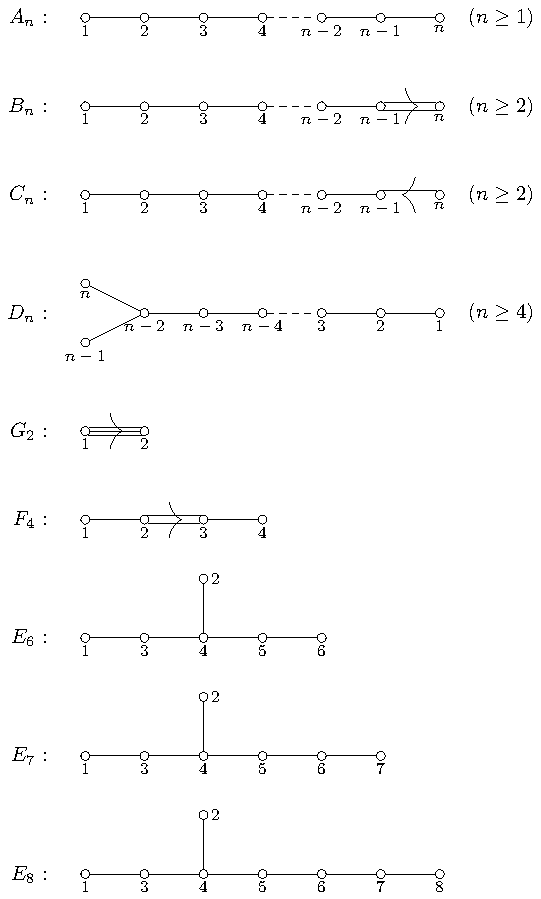
\includegraphics{graphics/positive_definite_graph.pdf}
  \end{center}
  \caption{正定値グラフ\label{fig:positive_definite_graph}}
\end{figure}

\begin{figure}[htbp]
  \begin{center}
    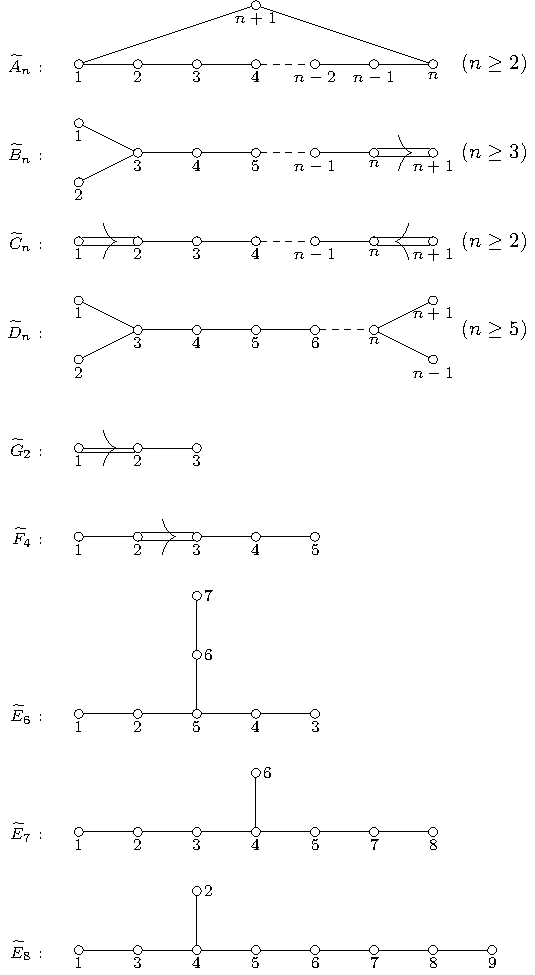
\includegraphics{graphics/non-positive_definite_graph.pdf}
  \end{center}
  \caption{非正定値グラフ\label{fig:non-positive_definite_graph}}
\end{figure}